% Copyright 2004 by Till Tantau <tantau@users.sourceforge.net>.
%
% In principle, this file can be redistributed and/or modified under
% the terms of the GNU Public License, version 2.
%
% However, this file is supposed to be a template to be modified
% for your own needs. For this reason, if you use this file as a
% template and not specifically distribute it as part of a another
% package/program, I grant the extra permission to freely copy and
% modify this file as you see fit and even to delete this copyright
% notice. 

\documentclass{beamer}

% There are many different themes available for Beamer. A comprehensive
% list with examples is given here:
% http://deic.uab.es/~iblanes/beamer_gallery/index_by_theme.html
% You can uncomment the themes below if you would like to use a different
% one:
%\usetheme{AnnArbor}
%\usetheme{Antibes}
%\usetheme{Bergen}
%\usetheme{Berkeley}
%\usetheme{Berlin}
%\usetheme{Boadilla}
%\usetheme{boxes}
%\usetheme{CambridgeUS}
%\usetheme{Copenhagen}
%\usetheme{Darmstadt}
%\usetheme{default}
%\usetheme{Frankfurt}
%\usetheme{Goettingen}
%\usetheme{Hannover}
%\usetheme{Ilmenau}
%\usetheme{JuanLesPins}
%\usetheme{Luebeck}
\usetheme{Madrid}
%\usetheme{Malmoe}
%\usetheme{Marburg}
%\usetheme{Montpellier}
%\usetheme{PaloAlto}
%\usetheme{Pittsburgh}
%\usetheme{Rochester}
%\usetheme{Singapore}
%\usetheme{Szeged}
%\usetheme{Warsaw}


\title{Docker}

\pgfdeclareimage[height=2.3cm]{cerc-logo}{cerc.png}
\pgfdeclareimage[height=0.6cm]{university-logo}{iiitd-logo.png}

% A subtitle is optional and this may be deleted
\subtitle{Why should I care ?}

\author{Muhammad Falak R~Wani \\ \inst{falakreyaz@gmail.com}} 

\institute[IIIT-D] % (optional, but mostly needed)
{
  Cybersecurity Education and Research Centre -- {\em (CERC)} \\
  Department of Computer Science\\
  IIIT-D\\
  \centering
  \pgfuseimage{cerc-logo}

}

\date{GDG DevFest "17}

\subject{Containers}

% If you have a file called "university-logo-filename.xxx", where xxx
% is a graphic format that can be processed by latex or pdflatex,
% resp., then you can add a logo as follows:

\logo{\pgfuseimage{university-logo}}

% Delete this, if you do not want the table of contents to pop up at
% the beginning of each subsection:
\AtBeginSubsection[]
{
	\begin{frame}<beamer>{Agenda}
		\tableofcontents[currentsection,currentsubsection]
	\end{frame}
}

% Let's get started
\begin{document}

\begin{frame}
	\titlepage
\end{frame}

\begin{frame}{Agenda}
	\tableofcontents
	% You might wish to add the option [pausesections]
\end{frame}

% Section and subsections will appear in the presentation overview
% and table of contents.
\section{Foundations}

\subsection{History}

\begin{frame}{Lets turn the dial back ...}{It started on 1979 }
	\Large{
	Finally we did realize it :
	\begin{itemize}
		\item {
				Bill Joy creates \textbf{chroot} in 1979.
			}
		\item {
				\textbf{VMware} joins in on 1998. (HW Virt)
			}
		\item {
				Solaris \textbf{Jails} in 2000. (OS  Virt)
			}
		\item {
				Solaris \textbf{Zones} in 2004. (Refinement of Jails)
			}
		\item {
				Google in 2007 \textbf{Process Containers} (\textbf{cgroups})

			}
		\item {
		        \textbf{LXC} was introduced in 2008
		
		}
		\item {
		        dotCloud Open Sourced \textbf{Docker} in 2013.
		}
	\end{itemize}
	}
\end{frame}

\subsection{Containers}

% You can reveal the parts of a slide one at a time
% with the \pause command:
\begin{frame}{What is a Container ?}{A boundary box}
{\Large Solution to the problem of how to \alert{get software to run reliably when moved} from one computing environment to another.}

\pause
\vfill{}
{\Large But wait! \\VM's also do the same...}
\end{frame}

\begin{frame}{A typical VM}{Very High overhead}
\begin{center}
    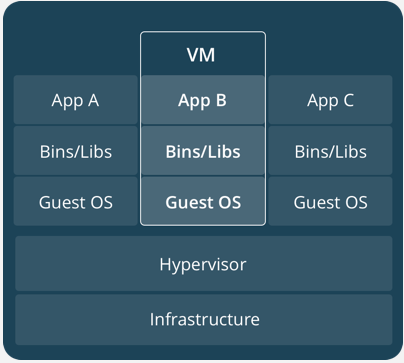
\includegraphics[height=6cm]{vm.png}
\end{center}
\end{frame}

\begin{frame}{A typical Container I}{Very Low overhead}
\begin{center}
    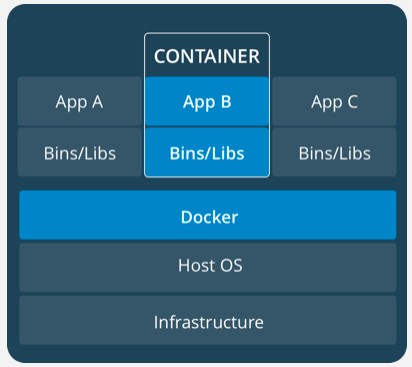
\includegraphics[height=6cm]{docker.png}
\end{center}
\end{frame}

\begin{frame}{A typical Container II}{How's it done ?}
    {\LARGE 
    \begin{itemize}
        \item \alert{namespaces}: Wraps a global system resource in an abstraction.
        \item \alert{cgroups}: Limits, accounts for, and isolates the resource usage.
    \end{itemize}
    }
    \vfill
    These are just pointers, so that you can look them up. Can't say much due to the time constraint.
\end{frame}



\subsection{Takeaways}
\begin{frame}{Advantages \& Disadvantages}{Lets draw a line}

{\Large 
\begin{itemize}
    \item \alert{Size}: VM's come with a lot of baggage (OS)
    \item \alert{Start-up Time}: A container uses your host OS, so starts almost instantly.
    \item \alert{Micro-Services}: Split the app in to modules. 
\end{itemize}
    \hrulefill
    
\begin{itemize}
    \item \alert{Can't} run a mix of OS's.
    \item \alert{Can't} work on the Kernel Level*.
\end{itemize}
}
\end{frame}

\begin{frame}{Hybrid Approach}{Best of both the worlds}
\begin{center}
    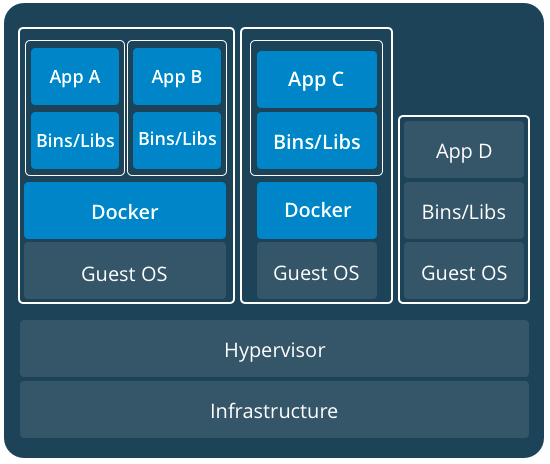
\includegraphics[height=6cm]{hybrid.png}
\end{center}
\end{frame}


\section{Docker 101}

\subsection{Current Trends}
\begin{frame}{Should I care ?}{You need to decide}
\begin{center}
    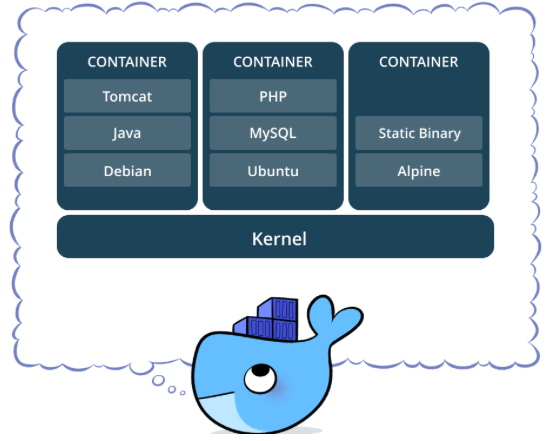
\includegraphics[height=6cm]{docker2.png}
\end{center}
\end{frame}

\begin{frame}{Should I care ?}{Obviously...}
\alert{Docker} will do the same to \alert{apt}, what \alert{apt} did to \alert{*.tar.gz}
	\begin{center}
        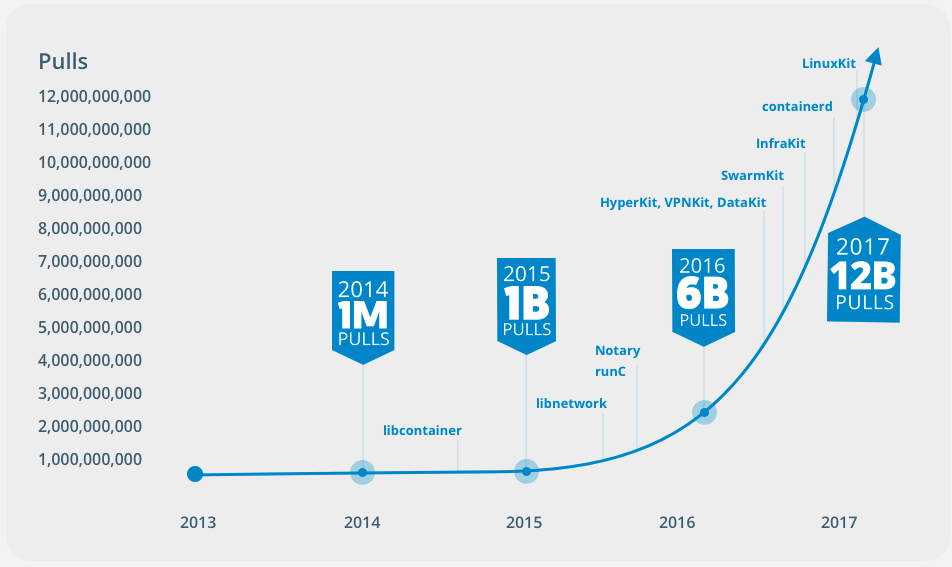
\includegraphics[height=5.6cm]{interest.png}
    \end{center}
\end{frame}


\subsection{Survival Skills}
\begin{frame}{Instantiate a Container}{docker container run}

{\Large 
docker \textit{container} \textbf{run} [options] \alert{image-name} \texttt{command} \\ -- or -- \\
docker \textbf{run} [options] \alert{image-name} \texttt{command} \\ 

\hrulefill
\begin{itemize}
    \item docker \textbf{run} \alert{hello-world}
    \item docker \textbf{run} \alert{alpine} \texttt{ping -c 5 www.google.com}
    \item docker \textbf{run} -d \alert{ubuntu} \texttt{sleep 600}
    \item docker \textbf{run} -it \alert{ubuntu} \texttt{bash}
\end{itemize}
}
\end{frame}
	
\begin{frame}{View Containers}{docker container ls}

{\Large 
docker \textit{container} \textbf{ls} [options]  \\ -- or -- \\
docker \textbf{ps} [options]  \\ 

\hrulefill
\begin{itemize}
    \item docker \alert{ps} 
    \item docker \alert{ps} -s
    \item docker \alert{ps} -a
    \item docker \alert{ps} -as
\end{itemize}
}
	
\end{frame}

\subsection{Basic Skills}

\begin{frame}{Miscellaneous I}{docker \{stop, start, remove, pull\}}

{\Large
\begin{itemize}
    \item \textbf{Stop} a running container:\\
    \texttt{docker \alert{stop} \#ash}
    
    \item \textbf{Start} a stopped container:\\
    \texttt{docker \alert{start} \#ash}
    
    \item \textbf{Remove} a stopped container:\\
    \texttt{docker \alert{rm} \#ash} \\
    \hrulefill
    
    \item \textbf{Pull} an Image from registry:\\
    \texttt{docker \alert{pull} image-name}
    
    \item \textbf{Remove} a docker image:\\
    \texttt{docker \alert{rmi} img-\#ash}
\end{itemize}
}
    
\end{frame}

\begin{frame}{Miscellaneous II}{docker \{stats, exec, attach, logs, inspect\}}
    
{\Large
\begin{itemize}
    \item Docker \textbf{stats} -- I/O, MEM, CPU:\\
    \texttt{docker \alert{stats} }
    
    \hrulefill
    
    \item \textbf{Exec} in a running container:\\
    \texttt{docker \alert{exec} \textbf{-it} \#ash}
    
    \item \textbf{Attach} to a detached container:\\
    \texttt{docker \alert{start} \#ash}
    
    \item \textbf{Logs} for a container:\\
    \texttt{docker \alert{rm} \#ash} 
    \item \textbf{Inspect} a container:\\
    \texttt{docker \alert{inspect} \#ash}\\
\end{itemize}
}
\end{frame}

\begin{frame}{Miscelaneous III}{Publishing ports \& Sharing files}
{\Large 
\begin{itemize}
    \item
    \textbf{Publishing Ports}: \\
    \texttt{docker run -it \alert{-p hPort:cPort} img cmd}\\
    
    \hrulefill
    
    \item \textbf{Sharing Files}: \\
    \texttt{docker run -it \alert{-v hPath:cPath} img cmd}
    
\end{itemize}
}
\end{frame}

\begin{frame}{Creating Docker Images}{docker commit \& Dockerfile}
    {\Large 
    \begin{itemize}
        \item \textbf{Saving}  container state:\\
        \texttt{docker \alert{commit} \#ash \textbf{tag}}\\
        \hrulefill
        \item \textbf{Dockerfile}:\\
        \texttt{docker \alert{build} \textbf{-t} tag /path/}
    \end{itemize}
    }
\end{frame}

\begin{frame}[fragile]{Dockerfile}{Creating docker Images}
\begin{verbatim}
FROM alpine:latest

LABEL maintainer "mfrw <falakreyaz@gmail.com>"

RUN apk --update add tor && adduser -D anon
COPY torrc /etc/tor/torrc

EXPOSE 9050 9051
USER anon

CMD [ "tor" ]
\end{verbatim}
    
\end{frame}
% Placing a * after \section means it will not show in the
% outline or table of contents.

\section*{Summary}

\begin{frame}{Summary}{Let's wrap it up}
{\Large 
\begin{itemize}
\item OS Level Virtualization.
\item Docker Images.
\item Docker pull/push
\item Docker Containers.
\item Dockerfile
\end{itemize}
}

\end{frame}

\end{document}

